% Setup
\graphicspath{./figures}

\chapter{Design and Implementation of a Service Mesh Benchmark}
\label{chap:system-design}

% Introduction
% - What will this chapter contain and what resaarch question it tries to answer

% Prev chapter -> General
% This chapter -> Perforormance oriented + importance
In the previous chapter (\cref{chap:survey}), we conducted a systems survey and identified several state-of-the-art \gls{sm} systems. We examined the architectural differences between these systems and compared them on domain-specific functional and non-functional requirements. We observed that architectural differences can have various effects on the theoretical performance implications such systems can have. Furthermore, the performance implications have great effects as they affect all software services in the environment. Therefore, we dive deeper into the performance of \gls{sm} systems.


% Which RQ will we answer
% Related work -> Shortcomings
% What we do to solve these shortcomings
In this chapter, we provide an answer to research question \ref{rq-2}. \textit{How to design and implement a \gls{sm} benchmark which evaluates the performance of \gls{sm} systems?} During the literature survey, we observed that there was no relevant work found in the \gls{pl}. Furthermore, preliminary research has shown that previous and current efforts made to evaluate these performance characteristics are either in early stages or have limited functionality. To solve these shortcomings, we present an extensible \gls{sm} benchmark instrument that aims to support various workloads, protocols and \gls{sm} implementations.

% Rest of the chapter is structured as follows
% - The need for these surveys (related work)
% - Methodology used for both surveys
% - Results of 
The remainder of this chapter is structured as follows. First, in \cref{sec:system:objectives} we introduce the goals of the benchmarking instrument. Second, in \cref{sec:system:sut} we describe the components that are part of the \gls{sut}. Afterwards, in \cref{sec:system:requirements-analysis} we present a requirement analysis in which we formalize the stakeholders, use cases and system requirements of the instrument. Next, in \cref{sec:system:design} we present the design of the benchmarking instrument. Following that, in \cref{sec:system:analysis} we analyse the proposed design.  Finally, in \cref{sec:system:implementation} we discuss the implementation details of the system.

\section{Benchmarking Objectives}
\label{sec:system:objectives}

% What are we trying to achieve with this benchmarking instrument
% - Analyize introduced latency
% - Analyze overhead in system resources CPU/mem
% - Analyze the maximum throughput of the system
% - Analyze protocol differences

The goal of a benchmarking instrument is to objectively compare, and decide on the best systems in a specific domain. However, the concrete definition of the best system depends on the underlying benchmarking objective \cite{folkerts2012benchmarking}. Therefore, it is important to first establish a set of goals for the benchmarking before designing or implementing it. In this section, we will introduce the benchmarking object vices, related to the main research question \ref{rq-2}.


To design a benchmark that evaluates key characteristics of a system, we guide the process by following industry best practices for measuring and monitoring distributed systems. Following the best practices and principles of the Google Site Reliability Engineering handbook \cite{google-sre}, we can establish a base set of metrics and signals that are important to measure in distributed systems. More specifically, we can follow the guidelines for \textit{white-box monitoring} and implement the  \textit{Four Golden Signals} in our benchmarking instrument.

The following list presents the objectives that the benchmarking instrument has.

\begin{enumerate}[label=\textbf{O\arabic*}, leftmargin=3\parindent]
    \item \textbf{Support System Resource Measurements}
    \label{o-1}
    
    The first objective of the benchmarking instrument is to measure the amount of system resources a \gls{sm} system uses.
    
    \item \textbf{Support Throughput Measurements}
    \label{o-2}
    
    The second objective is to measure the amount of throughput a system can handle. This is used to see if the \gls{sm} system introduces any bottleneck in terms of throughput.

    \item \textbf{Support Latency Measurements}
    \label{o-3}
    
    The third objective is to measure the amount of latency requests have. This is used to measure how much latency a \gls{sm} system introduces.
    

    \item \textbf{Support Resiliency Measurements}
    \label{o-4}
    The final objective of the instrument is to measure the resiliency of the systems by measuring the error rates within the system.
    
\end{enumerate}

\section{System Under Test}
\label{sec:system:sut}
% Explain SUT
% Components of Interest
% Purely Functional Components
% Present SUT

To design a benchmarking instrument that evaluates \gls{sm} systems, we first have to define the system and the components that are included in the benchmark. The components relevant to the benchmark are described in the \gls{sut}. However, even though the benchmark has to deal with numerous components in the system, not all are relevant to the benchmark.

Therefore, we split the components of the \gls{sut} in two categories according to the practices outlined by Folkerts et al. \cite{folkerts2012benchmarking}. The first group of components are labelled \textit{Components of Interest}. These components are of principal interest to the benchmark and have to be measured. The second group of components is labelled as \textit{Purely Functional Components}. The components in the latter group are present in the \gls{sut} in order for the benchmarking instrument to work correctly. However, measuring these components is not of importance relating to the objectives of the benchmark.

In \cref{fig:sut} we present the \gls{sut} for the benchmarking instrument. In the following sections, we elaborate on the  \textit{Components of Interest} (\cref{sec:system:sut:components-interest}) and \textit{Purely Functional Components} (\cref{sec:system:sut:components-functional})  present in this system.

\begin{figure}[!t]
    \centering
    
    \scalebox{.8}{    
    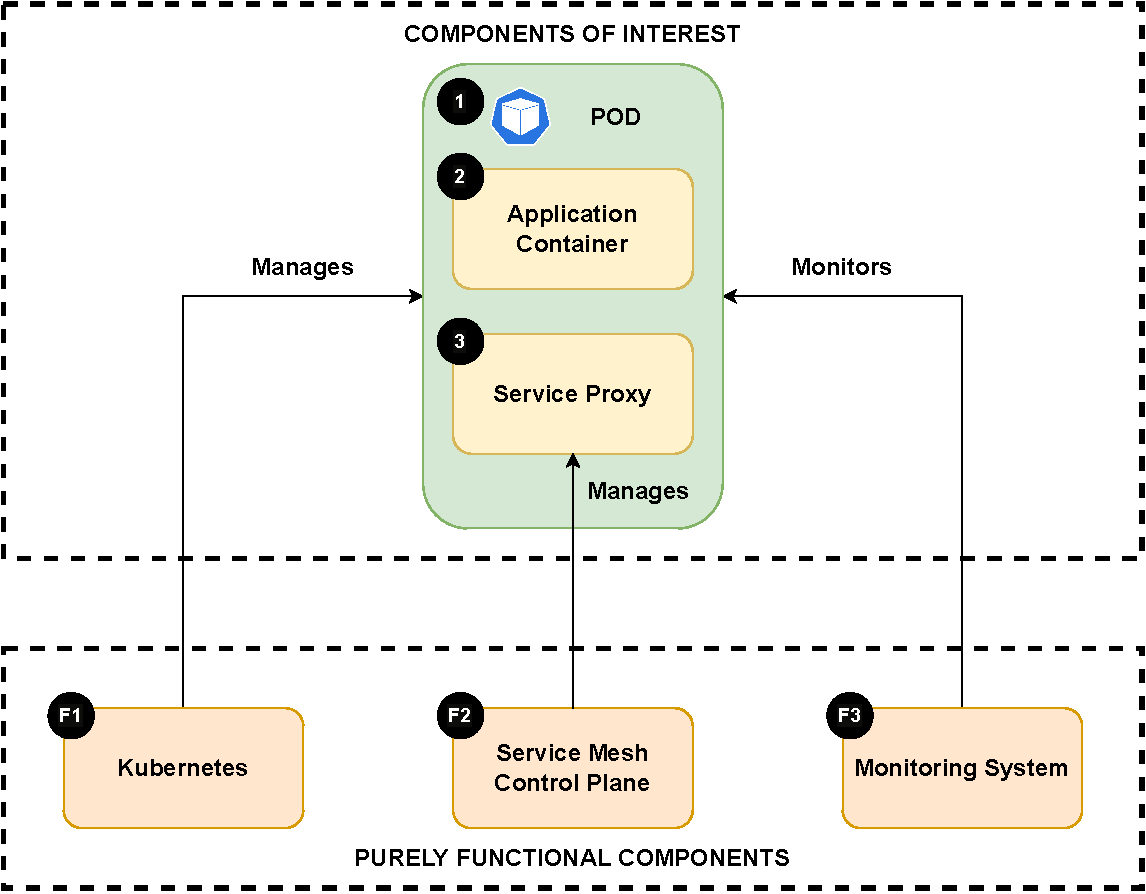
\includegraphics[width=\linewidth]{4_system_design/figures/system-under-test.pdf}
    }
    
    \caption{The \gls{sut} for benchmarking \gls{sm} systems.}
    
    \label{fig:sut}
\end{figure}

\subsection{Components of Interest}
\label{sec:system:sut:components-interest}
% Elaborate on the components of interest
% Data Path of Traffic
% Pod containing the service
% - Application Pod
% - Service Mesh Proxy (data plane)

The \textit{Components of Interest} are aligned with the objectives as presented in \cref{sec:system:objectives}. In the context of a \gls{sm} system, we aim to measure the components present in the data path of a software service. Therefore, in the context of a \gls{k8s} cluster running a \gls{sm} we evaluate the performance of software services that live in the \gls{k8s} specific abstraction, the \gls{pod} \designref{1}.

To measure the service and the service traffic, we measure the application container \designref{2} and the data plane component of a \gls{sm} \designref{3}.

\subsection{Purely Functional Components}
\label{sec:system:sut:components-functional}
% Elaborate on the functional components
% Metric Services - Prom
% Control Plane components of sm
% - More detail?

To be able to run the benchmark, we require the several components. First, we run the benchmark on a \gls{k8s} cluster \designref{F1}. Furthermore, a \gls{sm} system introduces several control plane components, which are required for the service mesh to correctly function \designref{F2}. However, since our objectives are to measure the data path of a \gls{sm} they are not of importance to the benchmarking instrument. Additionally, we introduce a metrics and monitoring system in the cluster \designref{F3}, which will be used to collect and time series data of the pods and containers residing in the \gls{k8s} cluster.
\section{Requirements Analysis}
\label{sec:system:requirements-analysis}

In this section, we expand on the details and requirements of the benchmarking instrument. To properly define the requirements of the benchmark, we first have to define the stakeholders and their use cases for such an instrument. After that is defined, we can define the actual requirements of the instrument based on those.

In \cref{sec:system:requirements-analysis:stakeholders} we define the stakeholders. Afterwards, in \cref{sec:system:requirements-analysis:use-cases} we define the use cases for the benchmarking instrument. Finally, in \cref{sec:system:requirements-analysis:requirements} we define the actual requirements.


\subsection{Stakeholders}
\label{sec:system:requirements-analysis:stakeholders}
% Who are the stakeholders?
% End users (cluster operators)
% Developers of SM platforms
% Scientific users

To uncover the use cases of this benchmarking instrument, we first have to identify the primary stakeholders. This is because stakeholders can have different applications for such a system, and therefore have different requirements. The following list of stakeholders (\ref{sh-1}-\ref{sh-3}) introduces the identified stakeholders and their concerns.

\begin{enumerate}[label=\textbf{S\arabic*}, leftmargin=3\parindent]
    \item \textbf{DevOps Engineers}
    \label{sh-1}
    
    This group of stakeholders is the primary user of a \gls{sm} system. They manage and control the infrastructure applications and services run on, and therefore can consider implementing a \gls{sm} system. Their primary concern with the benchmarking instrument is to evaluate the performance and resiliency characteristics of a \gls{sm} implementation on existing infrastructure or compare different implementations to make an informed decision to choose between the various implementations. For this group of stakeholders, it is important that the \gls{sm} matches their goals and requirement. This is exemplified by a DevOps engineer bound to predetermined \glspl{sla} that define contracts on service latencies.
    
    \item \textbf{Service Mesh Engineers}
    \label{sh-2}
    
    The second group of stakeholders consists of the engineers that develop the \gls{sm} systems itself. For these engineers, it is important to track the performance of their system to make sure that it meets the predetermined performance requirements. Furthermore, it can enable the engineers to compare their system to other offerings in the \gls{sm} landscape, which can help this group to set expectations and requirements.
    
    \item \textbf{Scientific Researchers}
    \label{sh-3}
    
    The final group of stakeholders represents researchers from academic institutions. This group uses the benchmarking instrument to conduct scientific research on the \gls{sm} systems, and their workloads. For this group of stakeholders, it is important that the benchmark instrument reports detailed information on both the system and the workloads running on it so that they can reason on the results.  Furthermore, it is important that the results the instrument produces are reproducible, meaning that experiments conducted with similar inputs produce similar outputs (bearing in mind the inherent variability in distributed environments). Finally, it is important that the instrument can run different workloads so that they can evaluate different situations and environments.
\end{enumerate}


\subsection{Use cases}
\label{sec:system:requirements-analysis:use-cases}
% What can this system be used for?
% https://www.similarweb.com/corp/blog/research/business-benchmarking/benchmarking-types/ -> Business benchmark translated to software
%  Competitive benchmarking –> See how one system compares to another
% Strategic benchmarking -> To look at the best performing system (in a category) to learn from
% Performance benchmarking -> Set targets of a system and evaluate over time
%  Validate Perforamnce Optimizations

Previously, we have identified the stakeholders of a benchmarking instrument, (\ref{sh-1}-\ref{sh-3}) as it is important to know the users and their concerns. This helps us to understand \textit{who} the users of the benchmark are, and \textit{why} they would use such an instrument.

To understand \textit{how} such a benchmark is used, we need to identify the use cases. Drawn from the concerns of the stakeholders, we present a list of use cases that (\ref{u-1}-\ref{u-3}) this benchmarking instrument can fulfil.

\begin{enumerate}[label=\textbf{UC\arabic*}, leftmargin=3\parindent]
    \item \textbf{Competitive Benchmarking}, \textit{concerns:} \ref{sh-1}, \ref{sh-2}, \ref{sh-3}
    \label{u-1}
    % Basic performance evaluation on multiple systems
    % Compare systems -> Which system is the best
    % Applies to: All
    
    The first and most common use case of the benchmarking instrument is to perform competitive benchmarking. The benchmarking instrument produces quantitative data on the performance characteristics of a \gls{sm} system.  The results of the benchmark can then be used to compare \gls{sm} implementations and decide on the best performing system in a domain.
    
    \item \textbf{Strategic Benchmarking}, \textit{concerns:} \ref{sh-2}, \ref{sh-3}
    \label{u-2}
    % Look at best system in category x
    % Look at the implementation details of that system (regarding category x)
    % Learn from it -> Apply
    % Applies to: Engineers, Academia
    
    \todo{Bench use case: mb rename strategic?}
    
    A second use case of the benchmarking instrument is to enable critical insights into the best performing systems. A benchmarking instrument gives insights into the performance of various characteristics of a system. This allows users to analyse the best performing systems in certain individual areas. Analysing those systems in further detail allows users to develop an understanding on how these systems achieved their results and allows them to learn from it. These critical insights can then be translated into other systems applying these best practices.
    
    \item \textbf{Evaluate Periodic Performance}, \textit{concerns:} \ref{sh-1}, \ref{sh-2}, \ref{sh-3}
    \label{u-3}
    % Compare the performance of a single system over time
    % Applies to: All
    
    A third use case for the benchmarking instrument is to capture the performance of a system over time. When conducting a benchmark, you evaluate a system and capture the performance of that system at a specific time. However, it can also be used to monitor and evaluate the performance of a system over a larger time frame to determine if, and by how much, the performance characteristics alter over time.
    
    
    \item \textbf{Validation of Performance Optimizations}, \textit{concerns:} \ref{sh-2}, \ref{sh-3}
    \label{u-4}
    % Developers -> Test changes to a sm system
    % See if perforamnce differs over versions
    % Applies to: Engineers, Academia

    Another use case for this benchmarking instrument is to analyse the impact of performance optimizations applied to \gls{sm} systems. When such an optimization is made, users can evaluate the system pre- and post-optimization to measure the impact of the optimization.
    

    \item \textbf{Validate System Requirements}, \textit{concerns:} \ref{sh-1}
    \label{u-5}
    % Evaluate if a sm implementation could be used in the environment oof the end user
    % e.g. SLA (min latency
    % Applies to: DevOps (end user)
    
    A final use case for this benchmarking instrument, is to evaluate if a \gls{sm} meets the requirements of the end user. End users can have different requirements, such as performance and resiliency requirements. This benchmark will enable those users to evaluate a \gls{sm} on their infrastructure to see if the system meets their requirements.
    
\end{enumerate}

\subsection{Requirements}
\label{sec:system:requirements-analysis:requirements}
% Introduce the requirements of the system
% Based on Folkters et al. three types of requirements
% - General Requirements
% - Implementation Requirements
% - Workload requirements

To design a benchmarking instrument that resembles any value, we satisfy the concerns and use cases of the identified stakeholders. To ensure that we satisfy this, we formulate a set of requirements, which we present in the following sections.

\subsubsection{Functional Requirements}
\label{sec:system:requirements-analysis:functional}

Functional requirements are requirements that the system \textit{must} implement, to function correctly. The following list (\ref{system:fr-1} - \ref{system:fr-7}) introduces the functional requirements of the benchmarking instrument and to which use case they relate.

\begin{enumerate}[label=\textbf{FR\arabic*}, leftmargin=3\parindent]
    \item \textbf{Support the most popular \gls{sm} implementations.}, \textit{related to:} \ref{u-1}, \ref{u-3}
    \label{system:fr-1}
    
    The benchmarking instrument must support the most popular \gls{sm} implementations. During the systems survey (\cref{chap:survey}), we identified that two of the identified \gls{sm} implementations currently dominate the landscape in terms of usage \cite{cncf-survey-2021}. Therefore, the benchmarking instrument has to support both \textit{Istio} and \textit{Linkerd} to be relevant for most users. 
    
    \item \textbf{Support systems using different data plane architectures}, \textit{related to:} \ref{u3}
    \label{system:fr-2}
    
    The benchmarking instrument must support all the identified data plane architectures (\cref{sec:survey:analysis:architectures}). During the systems survey, we identified four different data plane architectures with various performance implications. To analyse this, the benchmark must support at least one of the identified systems for each identified data plane architecture. The system already has to support systems adhering to the \textit{per-service} through the first established functional requirement (\ref{system:fr-1}). Since the other architectures only relate to a single \gls{sm} implementation, it means that the system must additionally support  \textit{Cilium} and \textit{Traefik}.
    
    \item \textbf{Implement and Report the Four Golden Signals}, \textit{related to:} \ref{u-1}, \ref{u-2}, \ref{u-3} 
    \label{system:fr-3}
    
    The benchmarking instrument must implement the \textit{Four Golden Signals}. To report meaningful data, we have to define meaningful metrics that the benchmarking instrument will report. To achieve this, we define the metrics by following industry best practices as established in the Google SRE handbook \cite{google-sre} and implement the \textit{Four Golden Signals}. This means that the benchmarking instrument must implement relevant metrics to report the \textit{Latency}, \textit{Traffic}, \textit{Errors}, and, \textit{Saturation} of the \gls{sut}.
    
    \item \textbf{Support Varying Workloads}, \textit{related to:} \ref{u-1}, \ref{u-3} 
    \label{system:fr-4}
    
    The benchmarking instrument must support varying workloads. This allows the benchmark to be relevant for the different use cases it can encounter and simulate the different workloads a \gls{sm} can see in the real world. To support this, the benchmark must provide a mechanism to specify the workload that the benchmark will run. Additionally, it has to provide a way in which the user can specify how the benchmark can extract relevant metrics. This is done by specifying how the workload, or service, can be consumed (e.g. HTTP endpoints).
    
    \item \textbf{Support Varying Cluster Environments}, \textit{related to:} \ref{u-1}, \ref{u-2}, \ref{u-3} 
    \label{system:fr-5}
    
    The benchmarking instrument must support varying cluster environments. This means that the benchmark must support any valid \gls{k8s} cluster environment. This allows users to evaluate \gls{sm} implementations on within their own environment and enables environment-specific use cases such as \ref{u-5}.
    
    \item \textbf{Report results in a well-known data format}, \textit{related to:} \ref{u-1}, \ref{u-2}, \ref{u-3} 
    \label{system:fr-6}
    
    The benchmarking instrument must report its results in a well-known data format. In order for the results to be useful to the various stakeholders, data must be presented in well-known formats such as \textit{JSON}, \textit{CSV} or \textit{YAML}.
    
    
    \item \textbf{Produce Reproducible Results}, \textit{related to:} \ref{u-1}, \ref{u-2}, \ref{u-3} 
    \label{system:fr-7}
    
    The benchmarking instrument must produce reproducible results. To provide meaningful results, the instrument has to be able to produce similar results when running a single experiment in the same environment. If the instrument is given the same inputs, similar outputs have to be expected.
    
\end{enumerate}


\section{Design of a Service Mesh Benchmarking Instrument}
\label{sec:system:design}

\section{Analysis}
\label{sec:system:analysis}

A benchmarking instrument is successful if all the stakeholders agree it provides meaningful results. To analyse if the proposed implementation satisfies this we use a set of guidelines established by Folkerts et al. \cite{folkerts2012benchmarking}. In their work they establish three groups of requirements which can be used to evaluate ea benchmarking instrument.

In the remainder of this section we introduce these three groups of requirements and evaluate them against the proposed benchmarking instrument. 

\section{General Requirements}
\label{sec:system:analysis:general}
% General Requirements – this group contains generic requirements.

The \textit{General Requirements} group establishes four broad requirements (\ref{gr-1} - \ref{gr-4}). The following list introduces those requirements and discusses how the proposed benchmarking instrument satisfies the conditions.

\begin{enumerate}[label=\textbf{GR\arabic*}, leftmargin=3\parindent]
    \item \textbf{Strong Target Audience}
    \label{gr-1}
    % The target audience must be
    % - considerable size and,
    % - interested to obtain the information.
    

    \item \textbf{Relevant}
    \label{gr-2}
    % The benchmark results have to measure the performance of the typical operation within the problem domain.
    

    \item \textbf{Economical}
    \label{gr-3}
    % The cost of running the benchmark should be affordable.
    

    \item \textbf{Simple}
    \label{gr-4}
    % The benchmark should be understandable, as it creates trust.
    
\end{enumerate}


\section{Implementation Requirements}
\label{sec:system:analysis:implementation}
% 2. Implementation Requirements – this group contains requirements regarding

The second group of requirements introduced in the work of Folkerts et al. is the \textit{Implementation Requirements} and establishes requirements (\ref{gr-1} - \ref{gr-4}). The following list introduces those requirements and discusses how the proposed benchmarking instrument satisfies the conditions.


\begin{enumerate}[label=\textbf{IR\arabic*}, leftmargin=3\parindent]
    \item \textbf{Fair and Portable}
    \label{ir-1}
    % All compared systems can participate equally.

    
    \item \textbf{Repeatable}
    \label{ir-2}
    % The benchmark results can be reproduced by rerunning the
    
    \item \textbf{Realistic and Comprehensive}
    \label{ir-3}
    % The workload exercises all SUT features typically used in the major classes of target application

    \item \textbf{Configurable}
    \label{ir-4}
    % a benchmark should provide a flexible performance analysis framework allowing users to configure and customize the workload.
\end{enumerate}


\section{Workload Requirements}
\label{sec:system:analysis:workload}
% 3. Workload Requirements – contains requirements regarding the workload definition and its interactions.
The final group of requirements introduced is the \textit{Workload Requirements} and consists of three requirements (\ref{wr-1} - \ref{wr-3}). The following list introduces those requirements and discusses how the proposed benchmarking instrument satisfies the conditions.

\begin{enumerate}[label=\textbf{WR\arabic*}, leftmargin=3\parindent]
    \item \textbf{Representativeness}
    \label{wr-1}
    % The benchmark should be based on a workload scenario that contains a representative set of interactions.
    
    \item \textbf{Scalable}
    \label{wr-2}
    % Scalability should be supported in a manner that preserves
    
    \item \textbf{Metric}
    \label{wr-3}
    % A meaningful and understandable metric is required to report about the SUT reactions to the load

\end{enumerate}
\section{Implementation}
\label{sec:system:implementation}

